\documentclass[a4paper,11pt, margin=1in]{article}
\usepackage[left=3cm, right=3cm, top=2cm]{geometry}
\usepackage[utf8]{inputenc}
\usepackage[formats]{listings}
\lstset{basicstyle=\ttfamily,
  showstringspaces=false,
  commentstyle=\color{red},
  keywordstyle=\color{blue}
}
\usepackage{pdfpages}
\usepackage[T1]{fontenc}


\renewcommand*\contentsname{Contenido}

\begin{document}


\newpage{}
\tableofcontents
\newpage{}

\section{Introducción}

El presente informe corresponde al trabajo práctico grupal \textbf{TP1} de la materia organización de computadoras.


\section{Documentación del diseño e implementación}
En el archivo main.c se usa a getopt para analizar los argumentos dados en la línea de comando y 
en base64.S se encuentra el código de codificación y decodificación en lenguaje MIPS32.


\subsection{{\normalsize Desarrollo de actividades}}

\begin{enumerate}
\item Se instala en un linux el emulador gxemul con NetBSD para realizar las pruebas.
\item Para el caso de la funcion de codificación fue necesario realizar un refactor para dividir mejor las tareas 
y facilitar la posterior traducción a MIPS32 assembly.
\item Se propuso antes de iniciar el desarrollo de cada función en MIPS32 assembly, estimar el tamaño de los 
stacks frames de las funciones que utilizan el base64\_encode y base64\_decode, 
respetando la convención de la ABI. 
\item Una vez que se programo ambas funciones en MIPS32 assembly, ambas funciones fueron incluidas en el main y
probadas en el ambiente de NetBSD instalado.
\item Para el debugging y corrección de errores se requirio utilizar el comando GDB
\begin{lstlisting}[language=bash,frame=\tiny]
$ gdb --args tp1 -a encode -i /root/envio/test.txt 
\end{lstlisting}
\item Para crear el presente informe se debe utilizar el comando pdflatex en el directorio informe.
\begin{lstlisting}[language=bash,frame=\tiny]
$ pdflatex informe_final.tex 
\end{lstlisting}

\end{enumerate}


\subsection{Menú (main.c)}
En  main.c se puede ver la implementación de un menú de ayuda, que posee una opción 
que ejecuta el programa en modo información "-h" que detalla las variantes de 
ejecución del programa, estas son -v que imprime la versión del programa y 
sale del mismo y otra es [options] que muestra las opciones disponibles; 
estas son -V, -h, -i que está disponible para indicar en donde se encuentra la dirección del archivo de entrada, 
-o lo mismo pero para el archivo de salida, 
-a que indica la acción que queremos que ejecute el programa, por default será encode 
y si quisiéramos que decodifique solo hace falta agregarle un decode.

Si se especifica la opción de codificar o decodificar entonces se podrá 
también especificar el archivo de entrada y de salida, se le podrá pasar un 
archivo especifico llamando a la función o también podrá pasárselo desde consola (Stdin y Stdout).

\newpage
\subsection{Codificación}
La codificación se hace posible con la agrupación de casos que conforman la solución, 
para esto se dividen los bytes en bits y se agrupan dependiendo de la llegada de los mismos; 
a cada caso le corresponde un respectiva máscara, un respectivo delta de desplazamiento, 
y los bits faltantes para completar con el signo "=". 
Los casos están ordenados, entonces con un bucle se irá codificando byte a byte. 
Esta codificación, agarra el caso y sus parámetros, busca en la tabla de base 64 
y traduce los bits en el carácter correspondiente. 
Finalmente, de ser necesario, completa la salida con caracteres de relleno.
\newline
Para la traducción a MIPS32 assembly fue necesario dividirlo en las siguientes funciones
\begin{enumerate}

\item base64\_encode: Función principal para la codificación.
\item calc\_indice: Calcula el indice para tabla de base 64.
\item escrib\_faltantes: Escribe los caracteres faltantes y los signos para completar.
\item escribir\_byte: Escribe un byte en el file descriptor indicado.

\end{enumerate}
A continuacion se muestra el stack frame de estas funciones:
\newline

%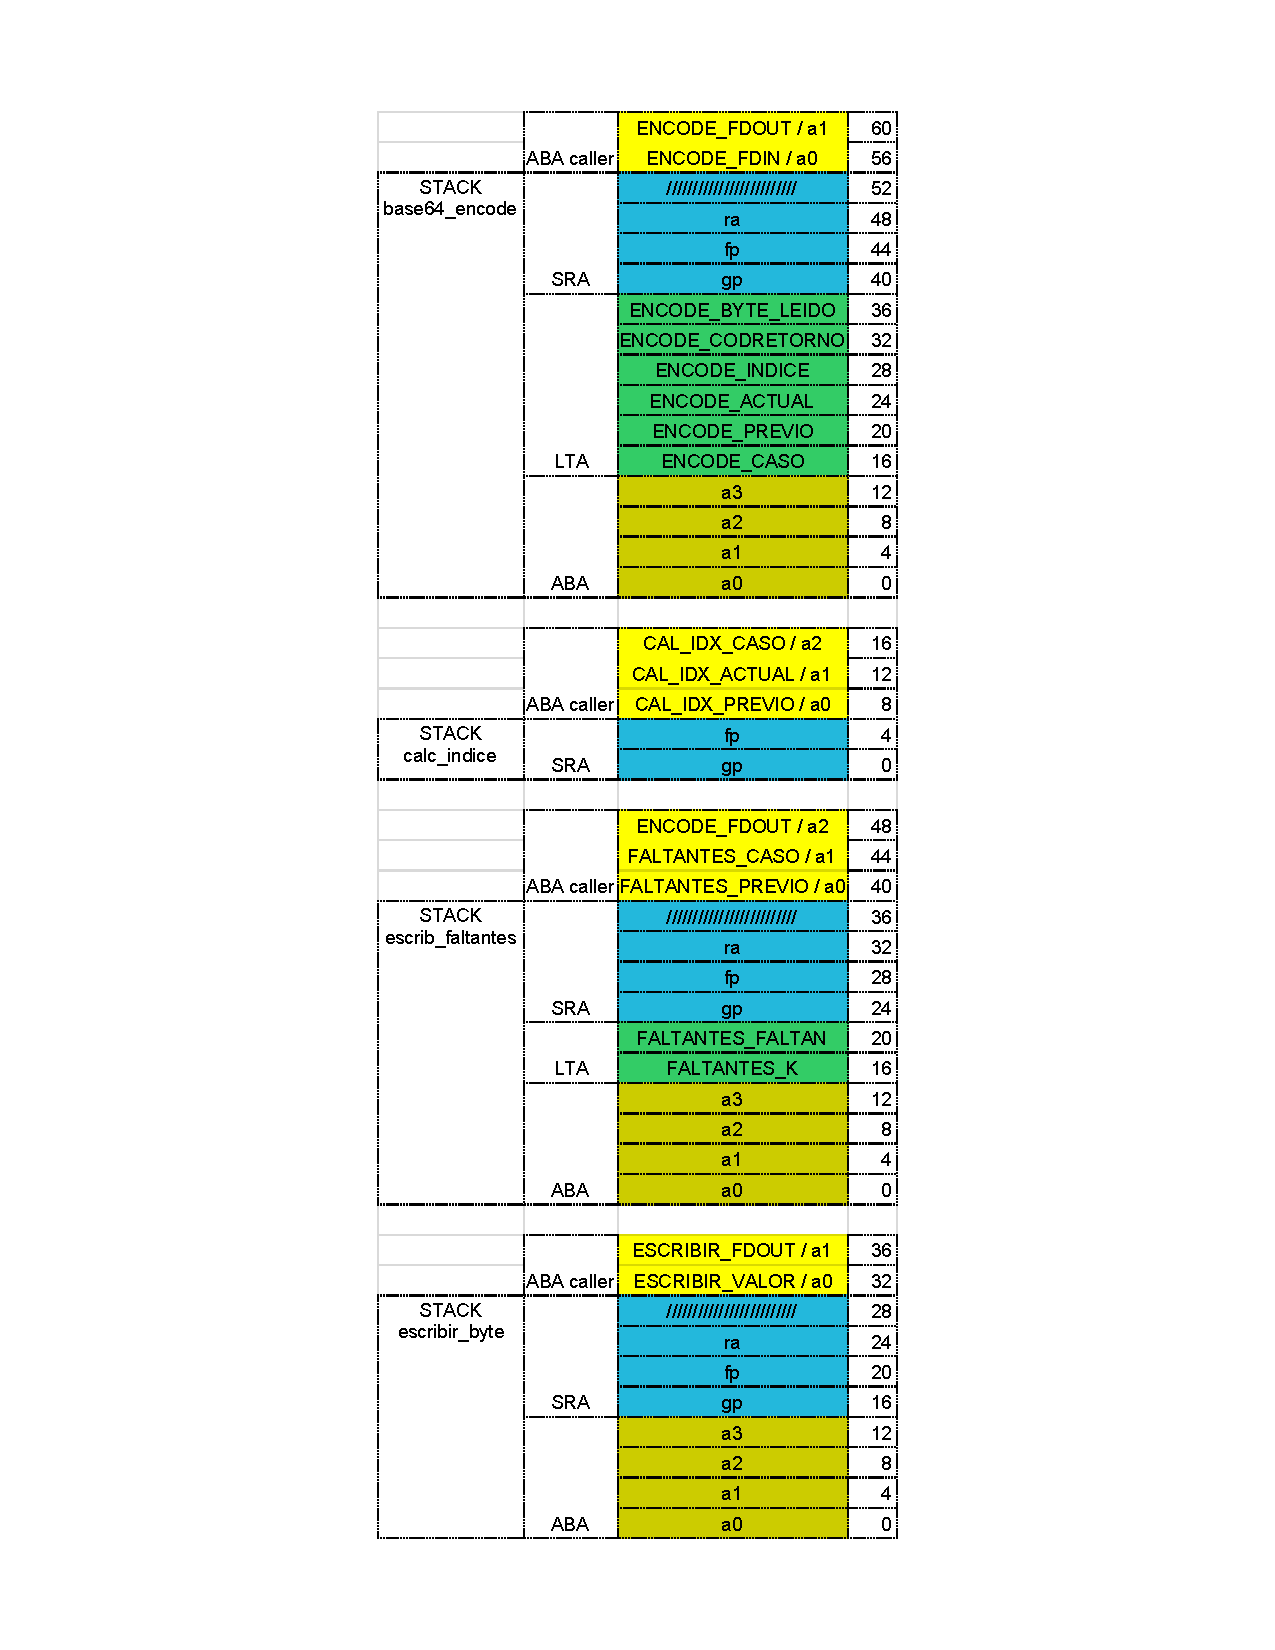
\includegraphics[width=0.8\textwidth]{stack_base64_encode.pdf}
	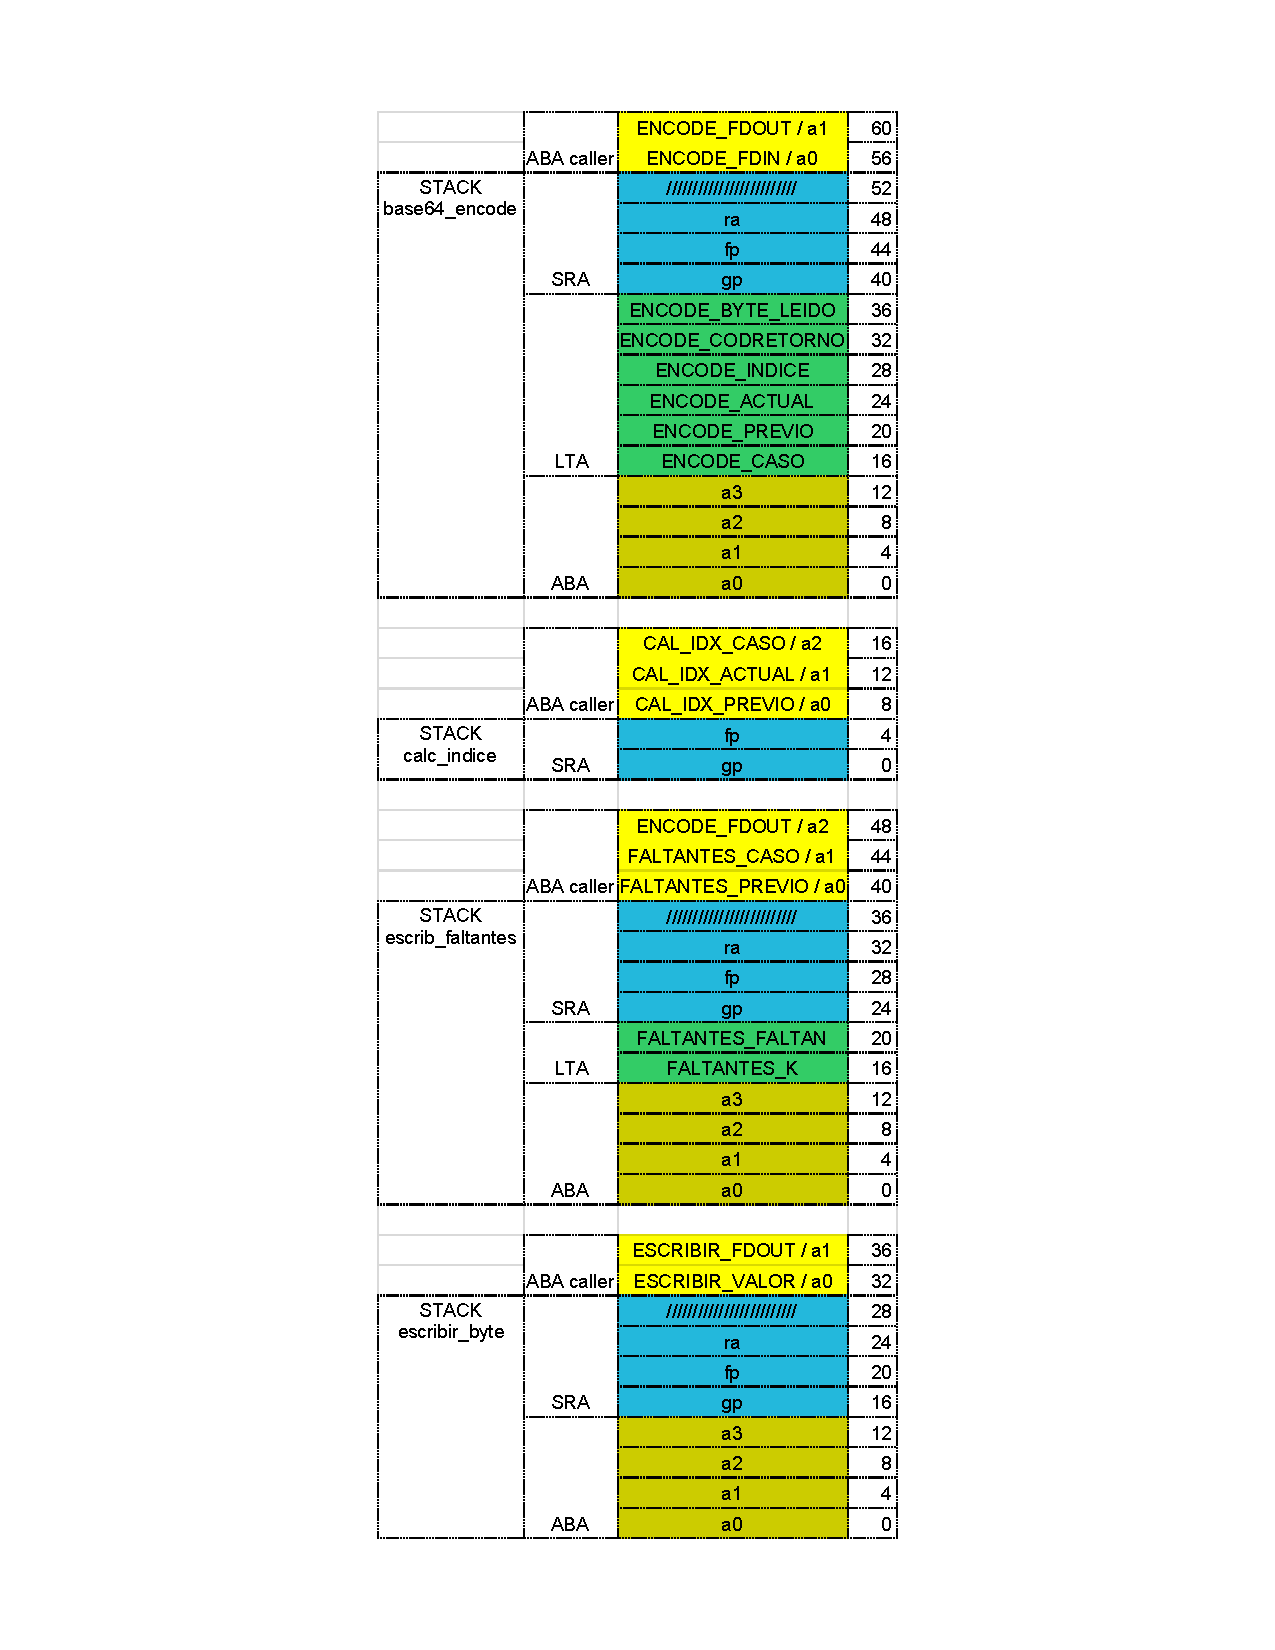
\includepdf[pages={1-},scale=1]{stack_base64_encode.pdf}

\subsection{Decodificación}
Se incluye una tabla de decodificación generada con la función crear\_tabla\_de\_decodificacion (incluida en el código), 
con ésta se podrán traducir los caracteres a decodificar a su índice dentro de la tabla de codificación, 
para de este modo poder concatenarlos y obtener la salida. Se tendrá en cuenta los caracteres inválidos, 
como por ejemplo '.', '!', etc o un '=' que no se encuentre en el lugar de caracter de relleno.
La decodificación se hará de a bloques de 4 bytes, aunque en principio se leen de a 5 bytes para estar 
seguros de que en los primeros 4 no habrá caracteres de relleno. 
El programa finaliza decodificando el final de la entrada, verificando que el número de caracteres de relleno 
sea el correcto.
\newline
Para la traducción a MIPS32 assembly fue necesario dividirlo en las siguientes funciones
\begin{enumerate}

\item base64\_decode: Función principal para la decodificación.
\item deco\_leer: Garantiza leer la cantidad de caracteres requeridos.
\item deco\_escribir\_char: Escribe un caracter a la salida.
\item deco\_resolver: Busca el caracter correspondiente en la tabla.
\item deco\_finales: Decodifica el final de la entrada y verifica el número de caracteres de relleno.

\end{enumerate}
A continuacion se muestra el stack frame de estas funciones:
\newline

%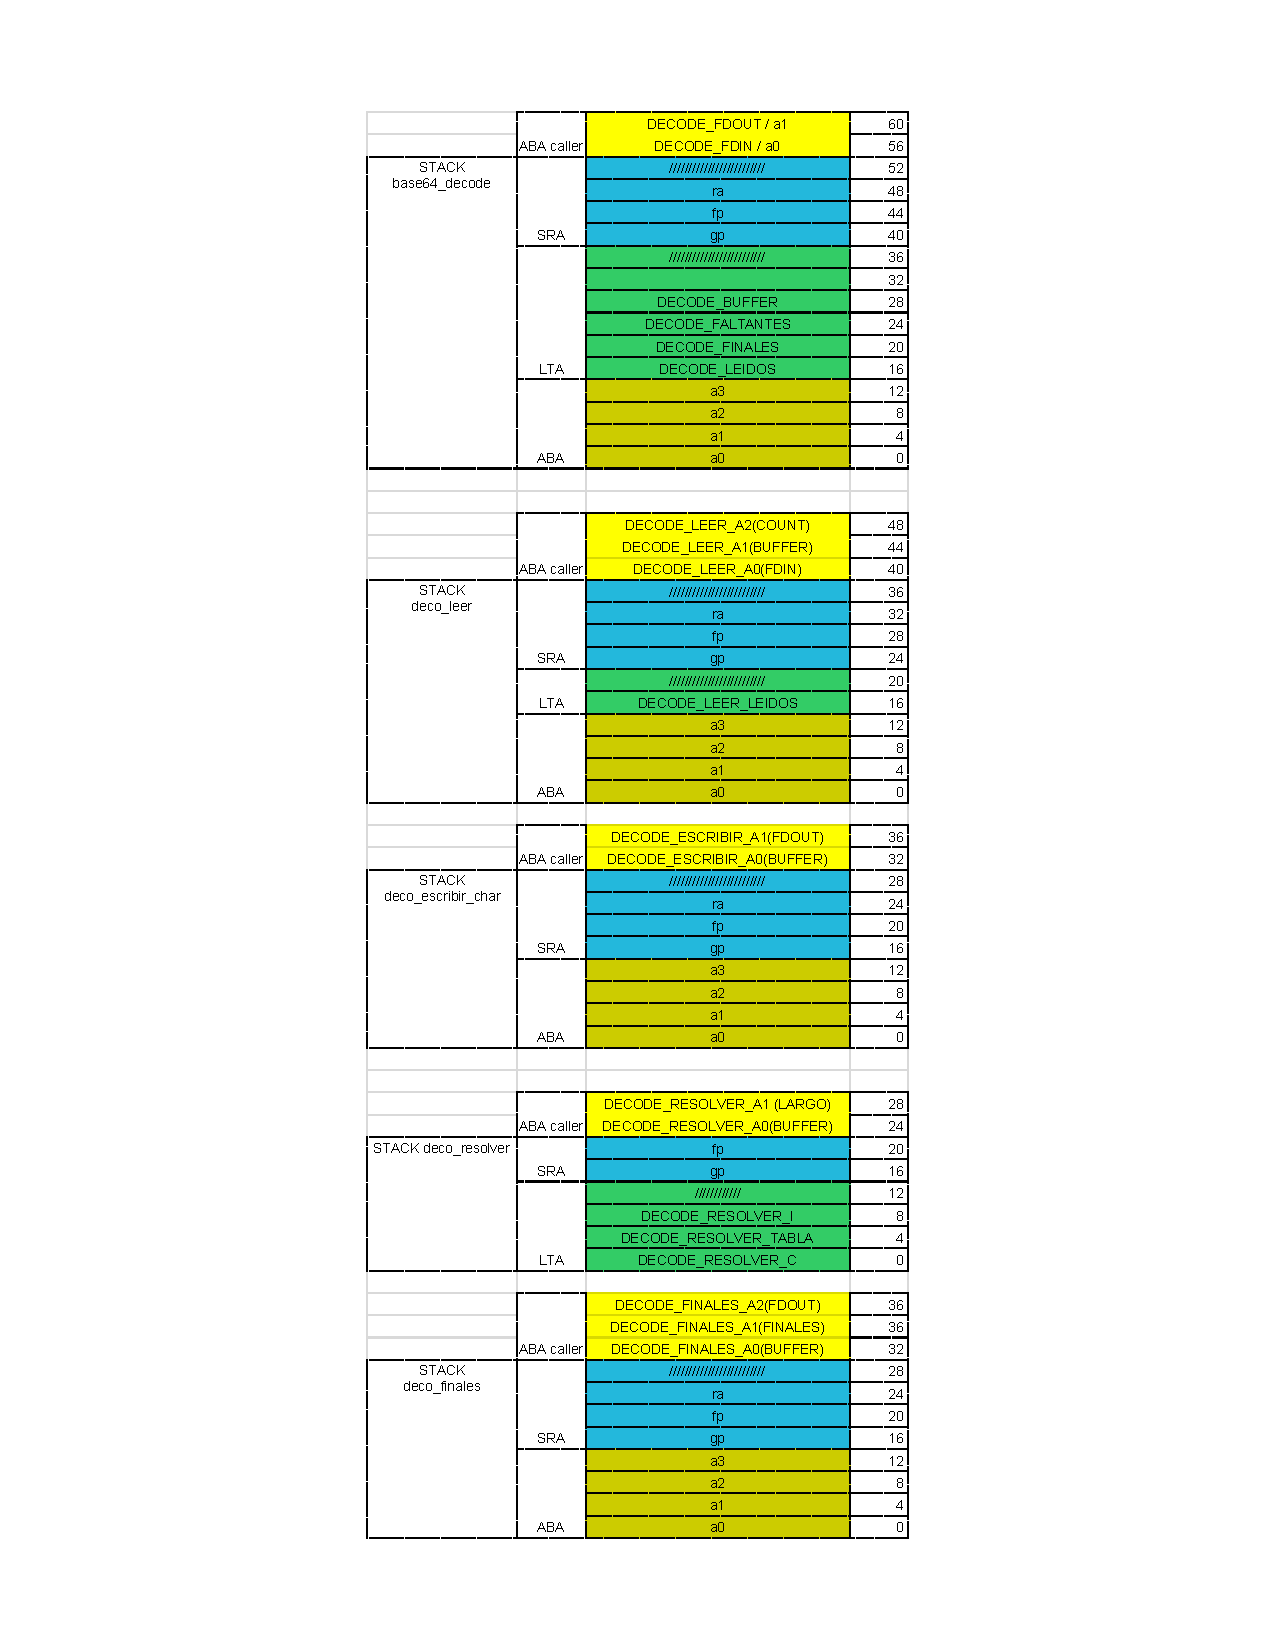
\includegraphics[width=0.8\textwidth]{stack_base64_decode.pdf}
	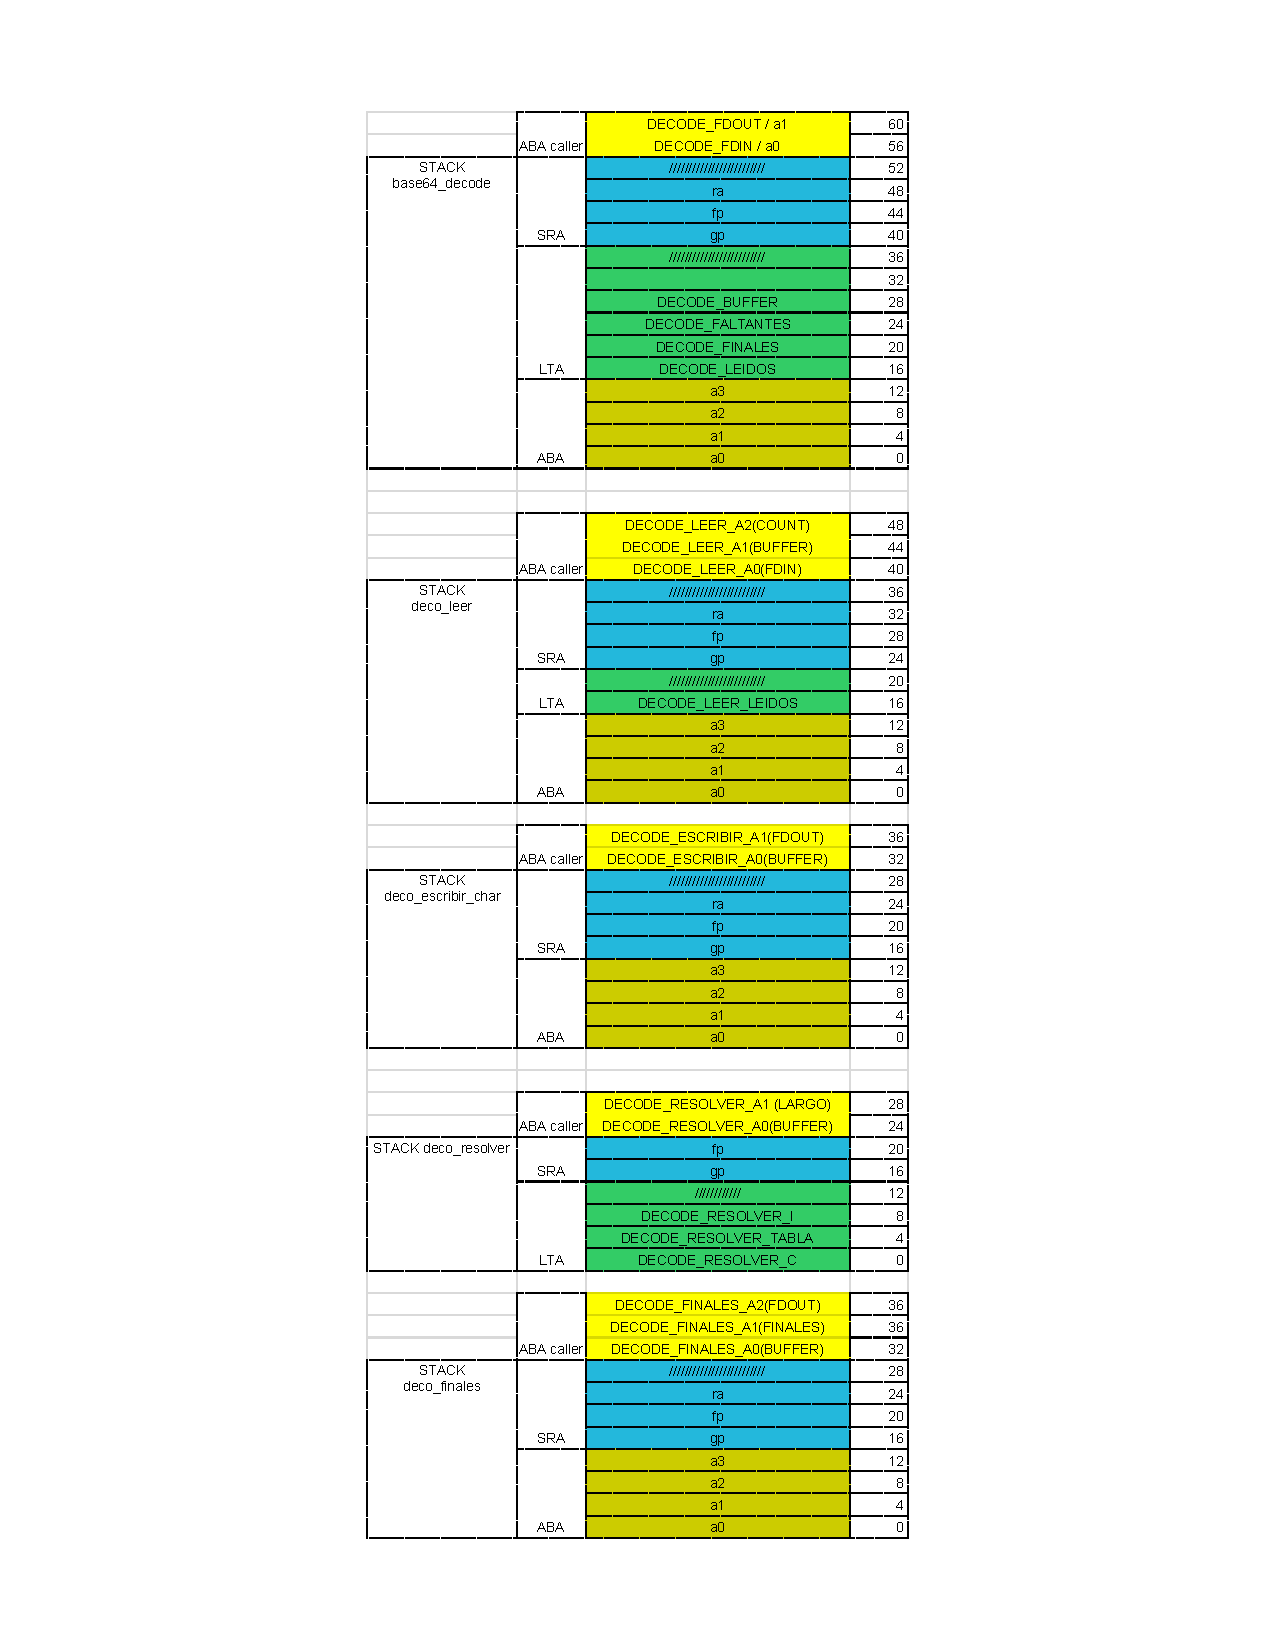
\includepdf[pages={1-},scale=1]{stack_base64_decode.pdf}


\subsection{Compilación}
Junto al código fuente se encuentra el Makefile de proyecto. La compilación debe realizarse dentro de la VM de NetBSD y
como resultado final generara un binario con el nombre tp1.

\begin{lstlisting}[language=bash,frame=\tiny]
$ make
\end{lstlisting}

\section{Pruebas}
\subsection{Código de pruebas.sh}
\begin{lstlisting}[language=c,breaklines=true]
#! /bin/sh

#Codificamos un archivo vacio (cantidad de bytes nula)
touch /tmp/zero.txt #creamos un archivo de texto vacio
./tp0 -a encode -i /tmp/zero.txt -o /tmp/zero.txt.b64
ls -l /tmp/zero.txt.b64
#-rw-r--r-- 1 user group 0 2018-09-08 16:21 /tmp/zero.txt.b64


#codificamos caracter ASCII M
echo -n M | ./tp0 
#TQ==
echo

#codificamos caracter ASCII M y a
echo -n Ma | ./tp0 
#TWE=
echo

echo "Test Codifico y decodifico una imagen. Prueba de binarios"
./tp0 -a encode -i recursos/linux-icon.png | ./tp0 -a decode -o recursos/linux-icon.png.b64 &&
      diff -s recursos/linux-icon.png recursos/linux-icon.png.b64

#codificamos Man
echo -n "Man" | ./tp0 
#TWFu
echo

#codificamos y decodificamos
echo Man | ./tp0 | ./tp0 -a decode
#Man
echo

#verificamos bit a bit
echo xyz | ./tp0 | ./tp0 -a decode | od -t c
#0000000 x y z \n
#0000004
echo
yes | head -c 1024 | ./tp0 -a encode #codificamos 1024 bytes, comprobamos longitud
#eQp5CnkKeQp5CnkKeQp5CnkKeQp5CnkKeQp5CnkKeQp5CnkKeQp5CnkKeQp5CnkKeQp5CnkK
#...
#eQp5CnkKeQp5CnkKeQp5CnkKeQp5CnkKeQp5CnkKeQp5CnkKeQp5CnkKeQp5CnkKeQp5Cg==
echo

#verificamos que los bytes sean 1024
yes | head -c 1024 | ./tp0 -a encode | ./tp0 -a decode | wc -c 
#1024
echo

#Generamos archivos de largo creciente, y verificamos que el procesamiento
de nuestro programa no altere los datos

n=1;
while :; do

head -c $n </dev/urandom >/tmp/in.bin;

./tp0 -a encode -i /tmp/in.bin -o /tmp/out.b64;

./tp0 -a decode -i /tmp/out.b64 -o /tmp/out.bin;

if diff /tmp/in.bin /tmp/out.bin; then :; else

echo ERROR: \$n;

break;

fi

echo ok: \$n;

n=\$((\$n+1));

rm -f /tmp/in.bin /tmp/out.b64 /tmp/out.bin
done
\end{lstlisting}

\subsection{Salida de pruebas.sh}
\begin{lstlisting}[language=c,breaklines=true]
-rw-r--r--  1 root  wheel  0 Oct 30 03:51 /tmp/zero.txt.b64
TQ==
TWE=
Test Codifico y decodifico una imagen. Prueba de binarios
Files recursos/linux-icon.png and recursos/linux-icon.png.b64 are identical
TWFu
Man


0000000   x   y   z  \n
0000004

eQp5CnkKeQp5CnkKeQp5CnkKeQp5CnkKeQp5CnkKeQp5CnkKeQp5CnkKeQp5CnkKeQp5CnkK
eQp5CnkKeQp5CnkKeQp5CnkKeQp5CnkKeQp5CnkKeQp5CnkKeQp5CnkKeQp5CnkKeQp5CnkK
eQp5CnkKeQp5CnkKeQp5CnkKeQp5CnkKeQp5CnkKeQp5CnkKeQp5CnkKeQp5CnkKeQp5CnkK
eQp5CnkKeQp5CnkKeQp5CnkKeQp5CnkKeQp5CnkKeQp5CnkKeQp5CnkKeQp5CnkKeQp5CnkK
eQp5CnkKeQp5CnkKeQp5CnkKeQp5CnkKeQp5CnkKeQp5CnkKeQp5CnkKeQp5CnkKeQp5CnkK
eQp5CnkKeQp5CnkKeQp5CnkKeQp5CnkKeQp5CnkKeQp5CnkKeQp5CnkKeQp5CnkKeQp5CnkK
eQp5CnkKeQp5CnkKeQp5CnkKeQp5CnkKeQp5CnkKeQp5CnkKeQp5CnkKeQp5CnkKeQp5CnkK
eQp5CnkKeQp5CnkKeQp5CnkKeQp5CnkKeQp5CnkKeQp5CnkKeQp5CnkKeQp5CnkKeQp5CnkK
eQp5CnkKeQp5CnkKeQp5CnkKeQp5CnkKeQp5CnkKeQp5CnkKeQp5CnkKeQp5CnkKeQp5CnkK
eQp5CnkKeQp5CnkKeQp5CnkKeQp5CnkKeQp5CnkKeQp5CnkKeQp5CnkKeQp5CnkKeQp5CnkK
eQp5CnkKeQp5CnkKeQp5CnkKeQp5CnkKeQp5CnkKeQp5CnkKeQp5CnkKeQp5CnkKeQp5CnkK
eQp5CnkKeQp5CnkKeQp5CnkKeQp5CnkKeQp5CnkKeQp5CnkKeQp5CnkKeQp5CnkKeQp5CnkK
eQp5CnkKeQp5CnkKeQp5CnkKeQp5CnkKeQp5CnkKeQp5CnkKeQp5CnkKeQp5CnkKeQp5CnkK
eQp5CnkKeQp5CnkKeQp5CnkKeQp5CnkKeQp5CnkKeQp5CnkKeQp5CnkKeQp5CnkKeQp5CnkK
eQp5CnkKeQp5CnkKeQp5CnkKeQp5CnkKeQp5CnkKeQp5CnkKeQp5CnkKeQp5CnkKeQp5CnkK
eQp5CnkKeQp5CnkKeQp5CnkKeQp5CnkKeQp5CnkKeQp5CnkKeQp5CnkKeQp5CnkKeQp5CnkK
eQp5CnkKeQp5CnkKeQp5CnkKeQp5CnkKeQp5CnkKeQp5CnkKeQp5CnkKeQp5CnkKeQp5CnkK
eQp5CnkKeQp5CnkKeQp5CnkKeQp5CnkKeQp5CnkKeQp5CnkKeQp5CnkKeQp5CnkKeQp5CnkK
eQp5CnkKeQp5CnkKeQp5CnkKeQp5CnkKeQp5CnkKeQp5CnkKeQp5CnkKeQp5CnkKeQp5Cg==
1024

ok: 1
ok: 2
ok: 3
ok: 4
ok: 5
[...]
\end{lstlisting}


\section{{\normalsize El codigo fuente, en lenguaje C}}

\subsection{main.c}

\lstinputlisting[language=C, basicstyle=\tiny]{../main.c}	

\subsection{base64.h}

\lstinputlisting[language=C, basicstyle=\tiny]{../base64.h}	

\section{{\normalsize Funciones de ENCODE/DECODE en codigo MIPS32}}

\lstinputlisting[language={[x86masm]Assembler}, firstline=1, lastline=1500, basicstyle=\tiny]{../base64.S}
 

\newpage
\section{{\normalsize Enunciado del trabajo practico}}

	%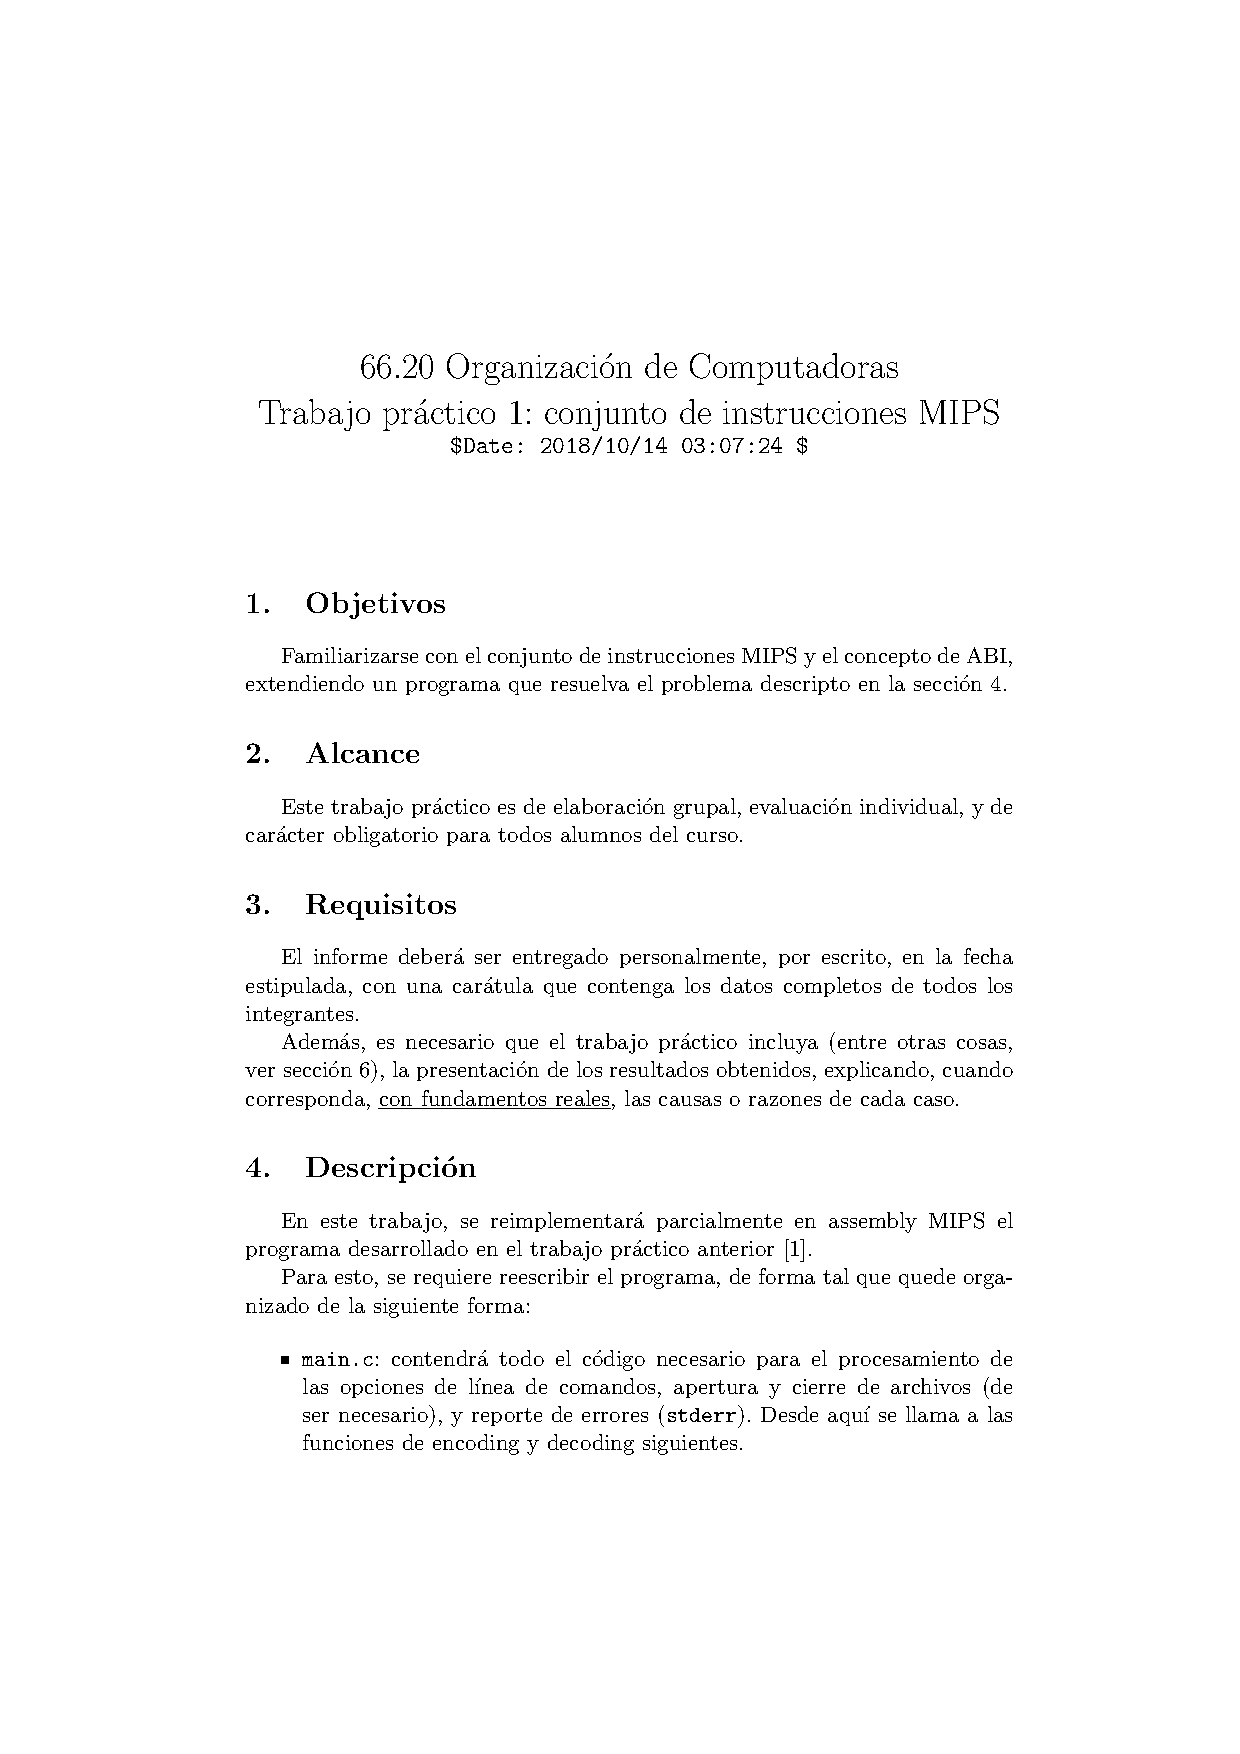
\includegraphics[width=0.8\textwidth]{tp1-2018-2q.pdf}
	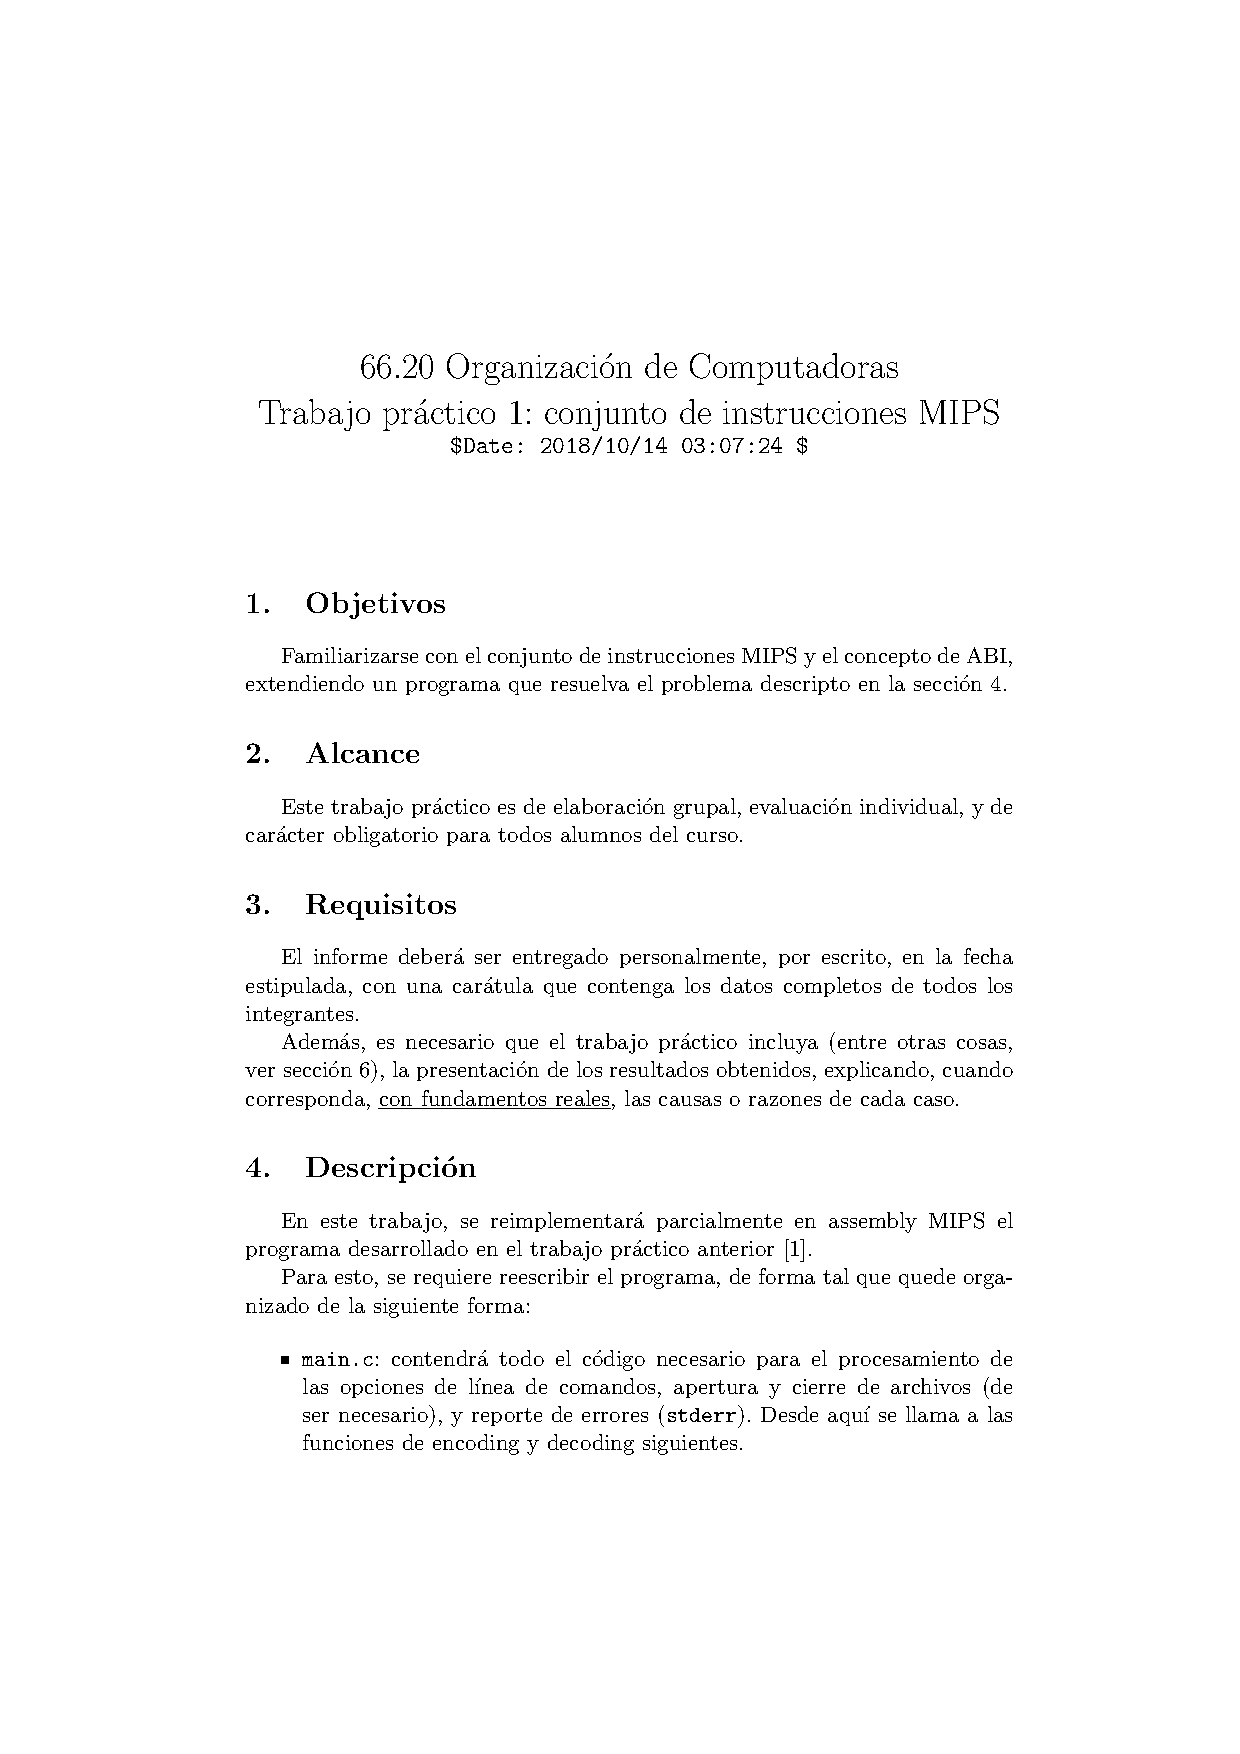
\includepdf[pages={1-},scale=1]{tp1-2018-2q.pdf}

\section{Conclusión}

Tuvimos problemas con los casos de prueba que involucraron pipes. Tuvimos que entender el funcionamiento de la
SYS\_read con pipes para poder solucionarlo. La solución fue leer hasta completar un buffer del tamaño esperado.
\newline
Se respetó las convenciones de la ABI para el desarrollo de las funciones en MIPS32, entendiendo que función es “leaf” y “non leaf” a la hora de definir el Stack Frame de cada una.
\newline
En cuanto al trabajo grupal en sí mismo, no hubo inconvenientes de
ningún tipo ya que al ser el grupo relativamente chico y tener conocimiento
del manejo del versionado de un proyecto ante cambios ingresado por
los integrantes (por medio del GIT), la introducción de modificaciones
y correcciones fui fluida.

\end{document}
